\documentclass[12pt]{report}

%%%%%%%%%%%%%%%%%%%%%%%%%%
%%%%%% UNIT PREAMBLE %%%%% 
%%%%%%%%%%%%%%%%%%%%%%%%%%

% Basics 
\usepackage[utf8]{inputenc}
\usepackage[T1]{fontenc}
\usepackage{textcomp}
\usepackage[a4paper, left=1in, right=1in, top=1in, bottom=1in]{geometry}
\renewcommand\familydefault{\sfdefault}

\usepackage[Sonny]{fncychap}

\usepackage{amsmath,amsfonts,amsthm,amssymb,mathtools}
\usepackage[varbb]{newpxmath}
\usepackage{xfrac}
\usepackage[usenames,dvipsnames]{xcolor} % usenames, dvipsnames adds more colours
\usepackage{hhline}
\usepackage{comment}
\usepackage{tasks}
\usepackage{enumerate} 
\usepackage{enumitem} 
\usepackage{titlesec}
\usepackage[most]{tcolorbox}
\usepackage{lipsum}
\usepackage{tabularx}
\usepackage[labelfont=bf]{caption}
\usepackage{subfig}
\usepackage{pgfplots}
\usepackage{cancel} 
\usepackage{physics} 
\usepackage[bookmarks]{hyperref}
\usepackage{array}
\usepackage{float}
\usepackage{standalone}
\usepackage{graphicx}
\usepackage{forest}

% Tables 
\numberwithin{table}{section}

% Inkscape Figures
\usepackage{import}
\usepackage{xifthen}
\usepackage{pdfpages}
\usepackage{transparent}
\newcommand{\incfig}[2][1]{
    \def\svgwidth{#1\columnwidth}
    \import{../figures/}{#2.pdf_tex}
}

\pdfsuppresswarningpagegroup=1

% Chemistry
\usepackage{lewis} 
\usepackage{bohr}
\usepackage[version=4]{mhchem}

% Page setup
\hypersetup{hidelinks}
\pagenumbering{arabic}
\pagestyle{plain}
\setlength{\parindent}{0pt}

% Show subsubsections
\setcounter{tocdepth}{3}
\setcounter{secnumdepth}{3}

% Required for the Grid
\usetikzlibrary{calc}

% Section Font-Size
\titleformat{\subsubsection}
  {\normalfont\fontsize{12}{12}\bfseries}{\thesubsubsection}{1em}{}

\titleformat{\subsection}
  {\normalfont\fontsize{14}{14}\bfseries}{\thesubsection}{1em}{}

\titleformat{\section}
  {\normalfont\fontsize{16}{16}\bfseries}{\thesection}{1em}{}

% New page for each section 
\newcommand{\sectionbreak}{\clearpage}

% Section Spacing
\titlespacing{\section}{0em}{2.5em}{1em}
\titlespacing{\subsection}{0em}{2.5em}{1em}
\titlespacing{\subsubsection}{0em}{2.5em}{1em}

% TABLE COLUMN SEPARATION (USES ARRAY PACKAGE)
% \renewcommand{\arraystretch}{1.8} % changes vertical space for each cell 
% \setlength{\tabcolsep}{18pt} % changes horizontal space for each cell
% \setlength{\arrayrulewidth}{0.25mm}

% TCOLORBOX 
% \newtcolorbox[auto counter, number within=section]{definition}{colback=white,title=Example~\thetcbcounter,breakable,colframe=white,boxrule=0pt, enhanced, title style={left color=gray!60,right color=white,middle color=white},arc=0mm, titlerule=0pt, fonttitle=\bfseries\sffamily}

% Theorems 
\usepackage{thmtools}
\usepackage[framemethod=TikZ]{mdframed}

\declaretheoremstyle[
    headfont=\bfseries\sffamily\color{ProcessBlue!70!black}, bodyfont=\normalfont,
    headpunct= :,
    mdframed={
        linewidth=2pt,
        rightline=false, topline=false, bottomline=false,
        linecolor=ProcessBlue, backgroundcolor=ProcessBlue!5,
        innerbottommargin=10pt
    } ]{note}

\declaretheoremstyle[
    headfont=\bfseries\sffamily\color{NavyBlue!70!black}, 
    bodyfont=\normalfont,
    % headpunct=,
    mdframed={
        linewidth=2pt,
        rightline=false, topline=false, bottomline=false, linecolor=NavyBlue, innerbottommargin=10pt
    }
]{solution}

\declaretheoremstyle[
    headfont=\bfseries\sffamily\color{Gray!70!black}, bodyfont=\normalfont,
    % headpunct= ,
    postheadspace=\newline,
    mdframed={
        linewidth=2pt,
        rightline=false, topline=false, bottomline=false,
        linecolor=Gray, backgroundcolor=Gray!5,
        innerbottommargin=10pt
    } ]{remark}

\declaretheoremstyle[
    headfont=\bfseries\sffamily\color{Fuchsia!70!black}, bodyfont=\normalfont,
    % headpunct= ,
    mdframed={
        linewidth=2pt,
        rightline=false, topline=false, bottomline=false,
        linecolor=Fuchsia, backgroundcolor=Fuchsia!5,
        innerbottommargin=10pt
    }
]{example}

\declaretheoremstyle[
    headfont=\bfseries\sffamily\color{Fuchsia!70!black}, 
    bodyfont=\normalfont,
    % headpunct= ,
    mdframed={
        linewidth=2pt,
        rightline=false, topline=false, bottomline=false,
        linecolor=Fuchsia,
    }
]{examplesolution}

\declaretheoremstyle[
    headfont=\bfseries\sffamily\color{black!70!black}, 
    bodyfont=\normalfont,
    mdframed={
        linewidth=1pt,
        rightline=false, topline=false, bottomline=false,
        linecolor=black,
    }
]{definition}

\declaretheorem[style=solution, name=Solution, numbered=no]{solution}

\declaretheorem[style=solution, name=Derivation, numbered=no]{derivation}

\declaretheorem[style=definition, name=Definition, numberwithin=chapter]{definition}

\declaretheorem[style=note, name=Note, numbered=no]{noteswap}
\newenvironment{note}[1]{\vspace{0.5em}\begin{noteswap}[#1]}{\end{noteswap}\vspace{0.5em}}

\declaretheorem[style=remark, name=Remark, numbered=no]{remarkswap}
\newenvironment{remark}{\vspace{0.5em}\begin{remarkswap}}{\end{remarkswap}\vspace{0.5em}}

\declaretheorem[style=example, name=Example, numbered=no]{exampleswap}
% \newenvironment{example}{\vspace{0.5em}\begin{exampleswap}}{\end{exampleswap}}

\declaretheorem[style=examplesolution, name=Solution, numbered=no]{examplesolutionswap}
\newenvironment{examplesolution}{\vspace{-2em}\begin{examplesolutionswap}}{\end{examplesolutionswap}}

% Enumerate environments 
\newenvironment{2qu}
{
\begin{enumerate}[label=(\alph*)]
}
{\end{enumerate}}

\newenvironment{3qu}
{
\begin{enumerate}[label=(\roman*)]
}
{\end{enumerate}}

% Normal Environments 
\newenvironment{list0.5}
{
\begin{enumerate}
\setlength\itemsep{0.5em}
}
{\end{enumerate}}

% \titleformat{\section}{\vbox{\rule{\linewidth}{0.8pt}}\bigskip\LARGE\bfseries}{\thesection}{1em}{}

\titleformat{\section}
  {\normalfont\Large\bfseries}{\thesection}{1em}{}[{\titlerule[0.8pt]}] % horizontal line below

% thmtools Environments
\newenvironment{problems}
{
    \subsection{Problems}
    \begin{enumerate}
    \setlength\itemsep{1em}
}
{\end{enumerate}}

\newenvironment{+problems}
{
    \subsubsection{Problems}
    \begin{enumerate}
    \setlength\itemsep{1em}
}
{\end{enumerate}}

\newenvironment{example}[1]
{
    \begin{exampleswap}
        #1
    \end{exampleswap}
    \begin{examplesolution}
}
{
\end{examplesolution}}

\newenvironment{2example}[1]
{
    \begin{exampleswap}[#1]
}
{
\end{exampleswap}}

% Managing Figures
\captionsetup{width=0.8\textwidth}
\renewcommand{\thefigure}{\arabic{chapter}.\arabic{figure}}

% TABLE
% \begin{table}[h!] % delete [h!] if there are bugs

%     %%% TABLE CONFIG %%% 
%     \renewcommand{\arraystretch}{1.5} % changes vertical space for each cell 
%     \setlength{\tabcolsep}{10pt} % changes horizontal space for each cell
%     \setlength{\arrayrulewidth}{0.25mm}

%     \begin{center}
%          title of the table \
%         \vspace{0.5em}
%         \begin{tabular}{|c|c|} % use r, l, c for right, left, center. use m{3cm} for middle width of 3cm, use  b{3cm} for bottom width of 3cm, and use p{3cm} for a top width of 3cm.  
%         \hline
%          &  \ % two columns corresponding to two c's
%         \hline
%          &  \ % second row
%         \hline
%         \end{tabular}
%     \end{center}
%     \caption{}
% \end{table}

% Symbols 
\newcommand{\z}{\mathbb{Z}}

\renewcommand{\l}{\ell}

% Formatting 
\newcommand{\invis}{\vphantom{Invisible Text}}
\newcommand{\divider}{\par\noindent\rule{\textwidth}{0.5pt}\vspace{0.4em}}

% Chemistry
% \newcommand{\2ch}[2]{\ce{#1}_{(#2)}}
% \newcommand{\io}[2]{\text{#1}^{#2}} 
% \newcommand{\2io}[3]{\text{#1}^{#2}_{#3}}


\begin{document}

\section{Questions}
\begin{enumerate}
\setlength\itemsep{1em}
    \item{What is the purpose of the cell cycle?}
        \begin{solution}
            \invis
            \begin{itemize}
                \item{Sustain the processes for cell division to occur.}
                \item{Cell growth; duplication of DNA and duplication of organelles.}
                \item{Maintain regular cell function.}
            \end{itemize}
        \end{solution}

    \item{Define the term ``interphase'' and describe its purpose.}
        \begin{solution}
            It refers to the period of time in which the cell carries out its regular cell functions. The purpose of interphase is to get the cell ready to divide (growth of the cell, duplication of the cell, duplication of DNA, duplication of organelles).
        \end{solution}

    \item{
        \begin{2qu}
            \item{What is mitosis?}
                \begin{solution}
                    This is when a single parent cell divides into two new daughter cells. The parent cells and daughter cells have the same DNA.
                \end{solution}
            \item{Why is mitosis important to the cell?}
                \begin{solution}
                    \textbf{Cell reproduction}; making new cells. \textbf{Growth}; optimization of cell surface area to cell volume ratio. High surface area to volume ratio is important. A high surface area to volume ratio maintains that nutrients can enter the cell efficiently and that waste can leave the cell efficiently.
                \end{solution}
        \end{2qu}}

        \item{Define and distinguish between the following terms: chromosomes, centromere, and sister chromatids.}
            \begin{solution}
                \invis
                \begin{itemize}
                    \item{ \textbf{Chromosome}: 
                            \begin{itemize}
                                \item{Genetic material.}
                                \item{Coiled version of cellular DNA called chromatin)}
                                \item{Comprised of sister chromatids.}
                            \end{itemize}
                        }
                    \item{ \textbf{Sister chromatids}:
                            \begin{itemize}
                                \item{Identical copies of DNA which are part of the chromosomes.}
                                \item{Attached at the center with a centromere during prophase and metaphase.}
                                \item{The sister chromatids are separated in mitosis during anaphase.}
                            \end{itemize}
                        \item{ \textbf{Centromere:}
                                \begin{itemize}
                                    \item{Holds the sister chromatids together during prophase and metaphase.}
                                    \item{2 sister chromatids attached by a centromere rom the chromosome.}
                                \end{itemize}
                            }
                        }
                \end{itemize}
                \begin{figure}[H]
                \centering
                    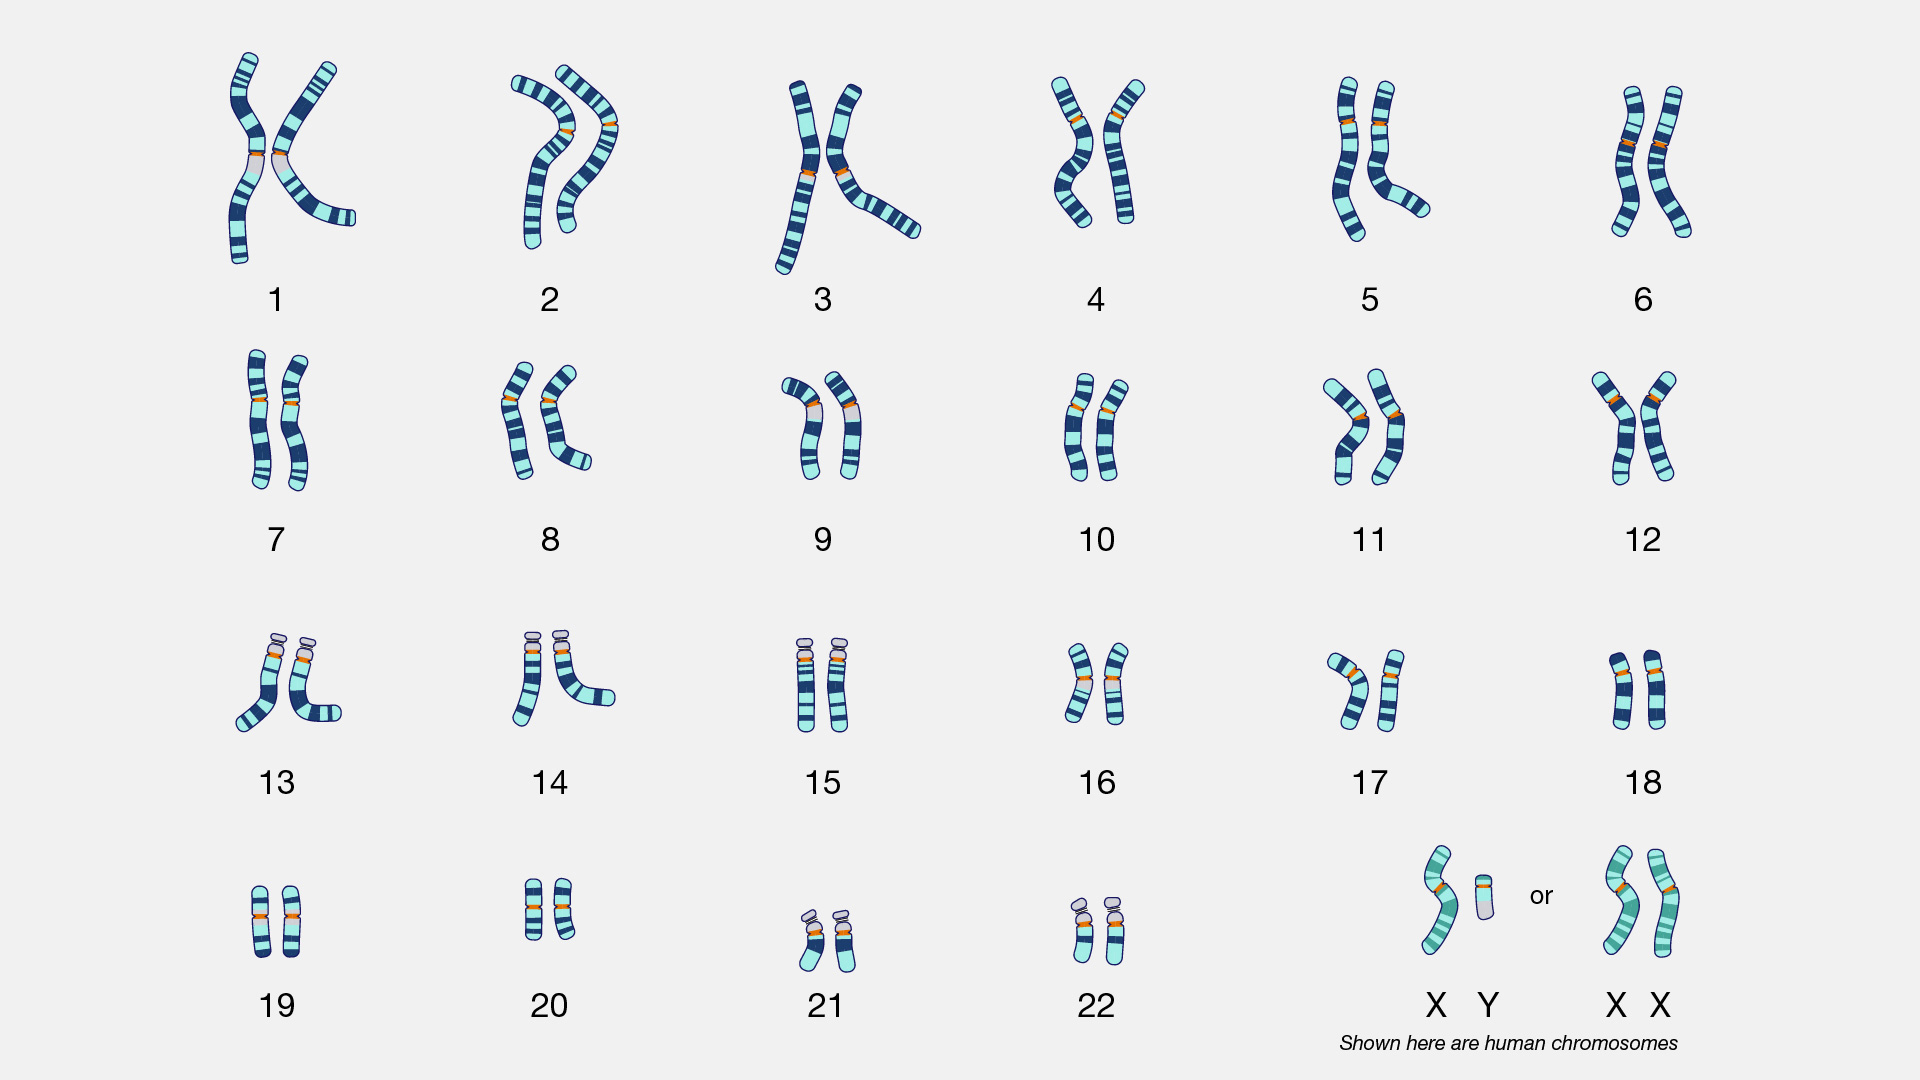
\includegraphics[width=\textwidth]{../figures/karyotype.jpg}
                    \caption{Karyotypes. In the bottom right, we see that there is XY or XX. The reason for this is because the one on the right (XY chromosome) is the male chromosome, and the one on the left (XX chromosome) is the female chromosome.}
                \end{figure}
            \end{solution}

            \item{Explain the meaning of cytokinesis.}
                \begin{solution}
                    \item{Happens after telephase. Is defined as the splitting/division of the cytoplasm. In an animal cell, this is done through the pinching of the membrane (we call this a cleavage furrow). In a plant cell, this is done through the formation of the cell plate.}
                        
                \end{solution}
\begin{figure}[ht]
    \centering
    \incfig[0.5]{animal-cell}
    \caption{Animal Cell vs Plant Cell}
    \label{fig:animal-cell}
\end{figure}
\end{enumerate}

\section{Healthy Cell Checkpoints}
\begin{definition}[Healthy Cell Checkpoints]
    A cell will not divide if 
    \begin{itemize}
        \item{Signals from surrounding cells tell the cell not to divide.}
        \item{Not enough nutrients for cell growth.}
        \item{DNA has not been replicated.}
        \item{DNA is damaged.}
    \end{itemize}
    Cell can undergo programmed cell death (apoptosis). See Figure \ref{fig:healthy-cell-checkpoints}. \\

    For more information, visit \url{https://www.khanacademy.org/science/ap-biology/cell-communication-and-cell-cycle/regulation-of-cell-cycle/a/cell-cycle-checkpoints-article}.
\end{definition}

\begin{figure}[H]
\centering
    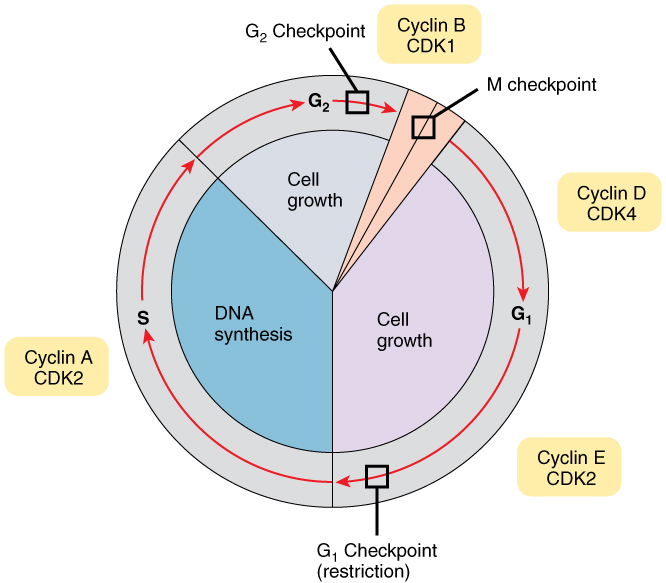
\includegraphics[width=0.9\textwidth]{../figures/healthy cell checkpoints.jpg}
    \caption{If a cell doesn't get the go-ahead cues it needs at the $G_1$ checkpoint, it may leave the cell cycle and enter a resting state called the \textbf{ $G_0$ phase}. Some cells stay permanently in $G_0$, while others resume dividing if conditions improve.}
    \label{fig:healthy-cell-checkpoints}
\end{figure}

\subsection{$G_1$ Checkpoint}
\begin{definition}[$G_1$ Checkpoint]
    The main decision point for a cell; that is, the primary point at which it must choose whether or not to divide. Once the cell passes the $G_1$ checkpoint and enters S phase, it becomes ireversibly committed to division. See Figure \ref{fig:g1-g2-checkpoints}.
\end{definition}

\subsection{$G_2$ Checkpoint}
\begin{definition}[$G_2$ Checkpoint]
    At this stage, the cell will check: 
    \begin{itemize}
        \item{ \textbf{DNA integrity}: is any of the DNA damaged?}
        \item{ \textbf{DNA replication}: was the DNA completely copied during S phase?}
            If there is damage, the cell will stall at the $G_2$ phase to repair. If the damage is unrepairable, the cell will undergo apoptosis (self destruction). See Figure \ref{fig:g1-g2-checkpoints}.
    \end{itemize}
\end{definition}

\begin{figure}[!htb] 
    \centering
    \subfloat[\centering $G_1$ checkpoint.]{{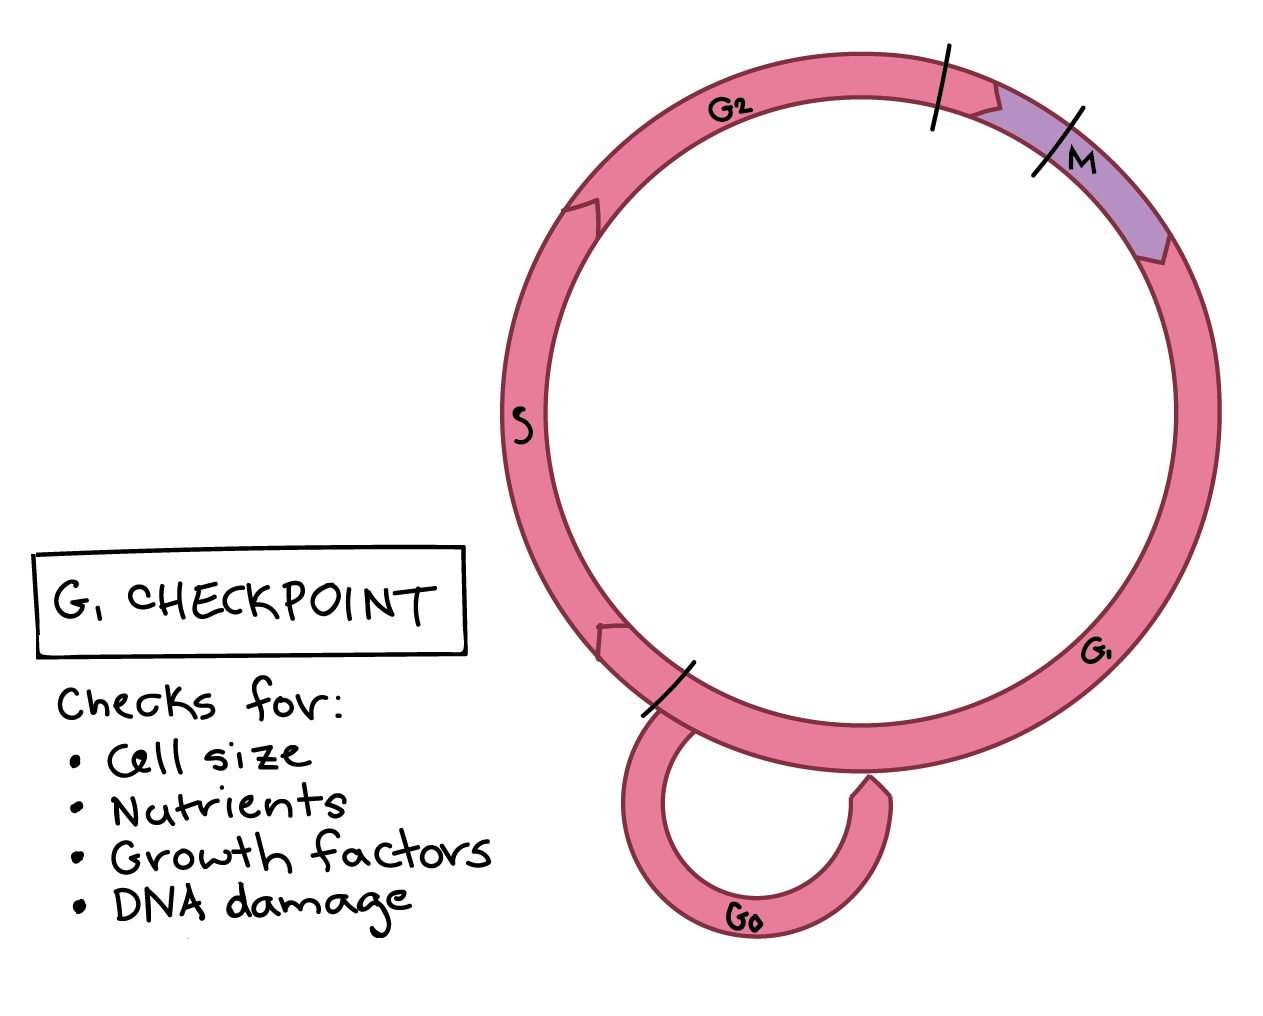
\includegraphics[width=0.45\textwidth]{../figures/g1 checkpoint.png}}}  
    \qquad
    \subfloat[\centering $G_2$ checkpoint.]{{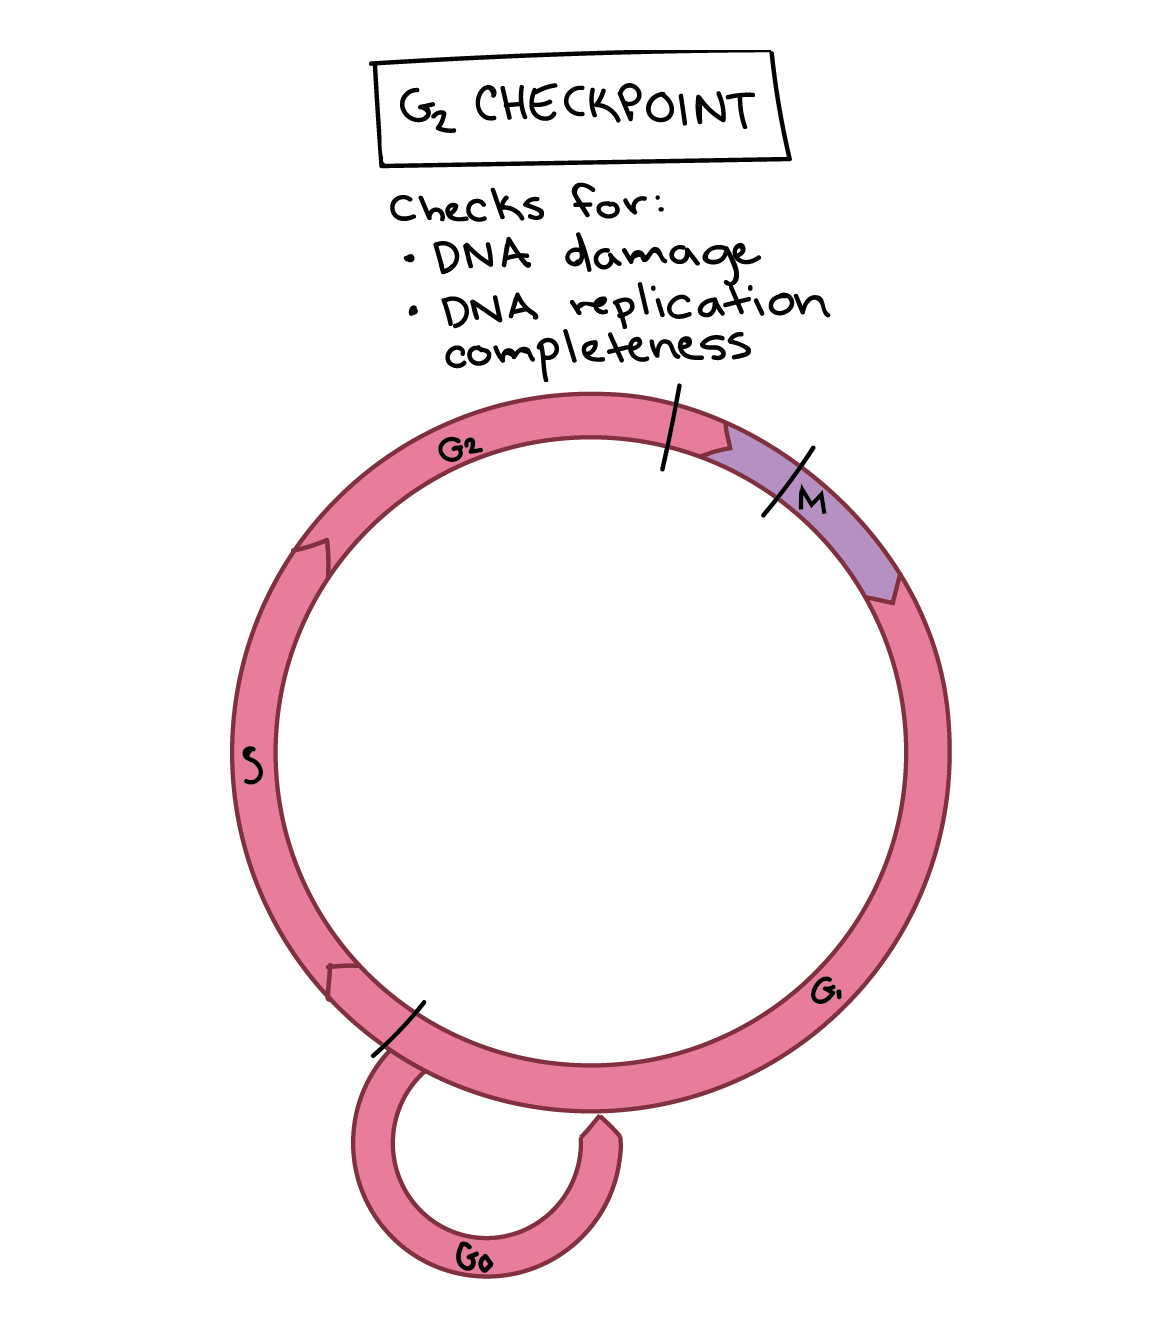
\includegraphics[width=0.45\textwidth]{../figures/g2 checkpoint.png}}}  
    \label{fig:g1-g2-checkpoints}
    \caption{The $G_1$ and $G_2$ checkpoints.}
\end{figure}

\subsection{The Spindle Checkpoint}
\begin{definition}[The Spindle Checkpoint]
    The M checkpoint is known as the ``spindle checkpoint''. Here, the cell examines whether all the sister chromatids are correctly attached to the spindle microtubles. See Figure \ref{fig:m-checkpoint}.
\end{definition}

\begin{figure}[H]
\centering
    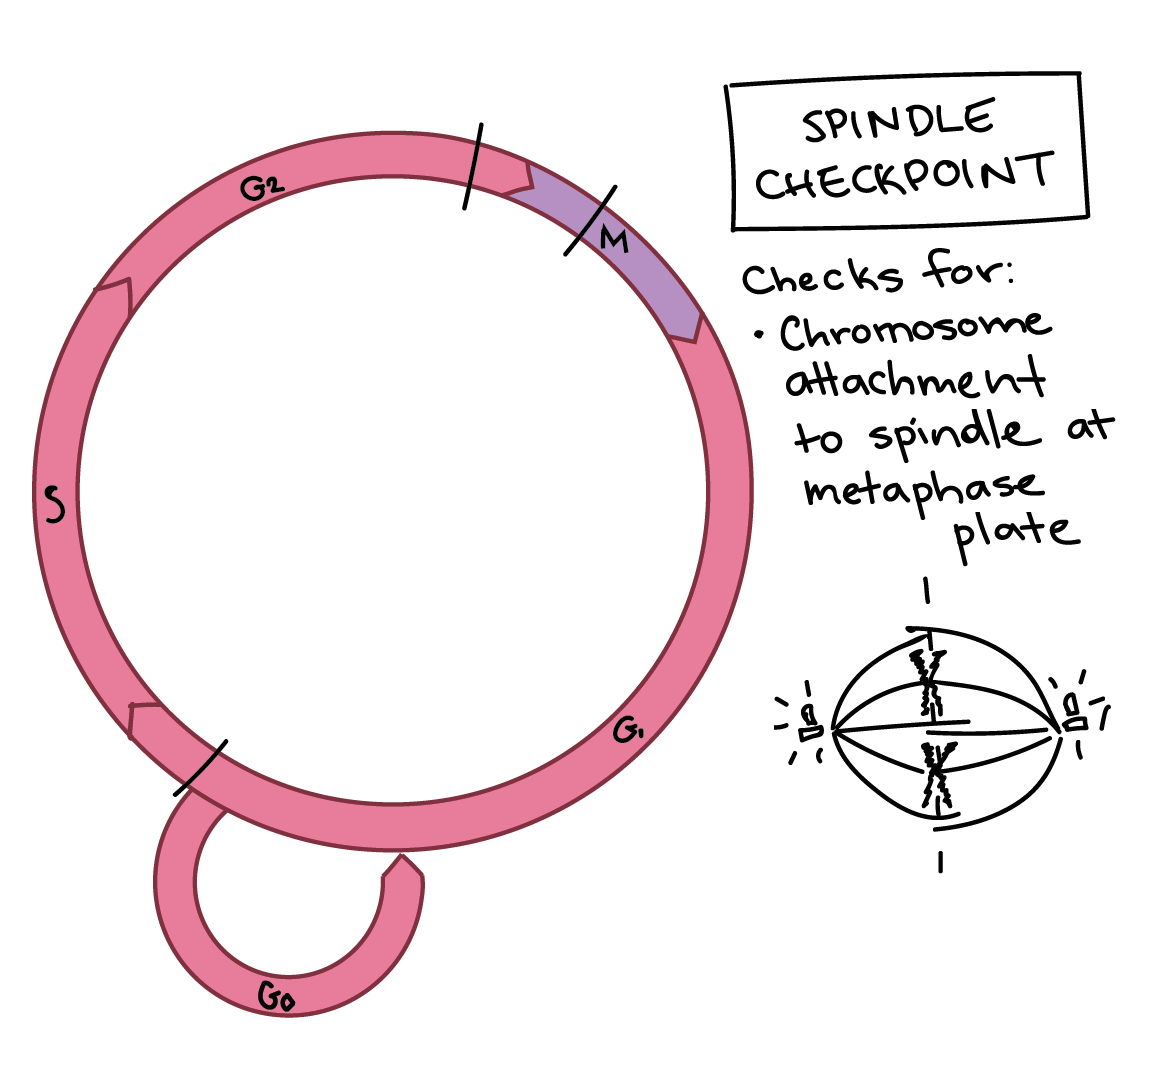
\includegraphics[width=0.45 \textwidth ]{../figures/m checkpoint.png}
    \caption{The spindle checkpoint (M checkpoint).}
    \label{fig:m-checkpoint}
\end{figure}

\section{Cancer}
\begin{definition}[Cancer]
    This is a group of diseases in which cells grow and divides uncontrollably. See Figure \ref{fig:cancer} and Table \ref{table:cancer-vs-normal}.
\end{definition}

This is caused by mutations to the DNA within cells which can allow rapidgrowth, fail to stop uncontrolled cell growth, or make errors when correcting DNA. Mutations are inherited or caused by environmental factors (i.e. radiation, viruses, carcinogens, etc.).

\begin{figure}[H]
\centering
    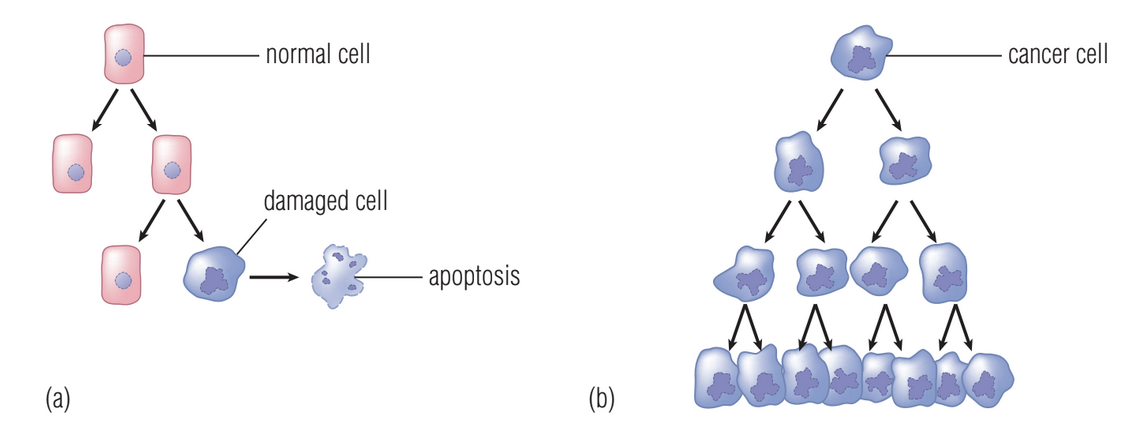
\includegraphics[width=0.75\textwidth]{../figures/cancer.png}
    \caption{(a) Cell division and cell death in normal cells. (b) Cell division in cancer cells.}
    \label{fig:cancer}
\end{figure}

\subsection{Stages of Cancer}
% TODO
\textbf{Stage 0}: cancer cells remain in place to form a mass cells called a tumour.\\ 
\textbf{Stage 1:} small tumour has not grown deeply into nearby tissues and has not spread to lymph nodes.\\ 
\textbf{Stage 2 $\&$ 3:} larger tumours have grown deeply into nearby tissue and may have spread to lymph nodes.\\
\textbf{Stage 4:} cancer has spread to other organs or parts of the body (metastasis).

\begin{table}[h!] % delete [h!] if there are bugs

    %%% TABLE CONFIG %%% 
    \renewcommand{\arraystretch}{1.5} % changes vertical space for each cell 
    \setlength{\tabcolsep}{10pt} % changes horizontal space for each cell
    \setlength{\arrayrulewidth}{0.25mm}

    \begin{center}
        Colorectal Cancer 5 year survival rates \\
        \vspace{0.5em}
        \begin{tabular}{|c c|} % use r, l, c for right, left, center. use m{3cm} for middle width of 3cm, use  b{3cm} for bottom width of 3cm, and use p{3cm} for a top width of 3cm.  
        \hline
        Stage & Survival Rate \\ % two columns corresponding to two c's
        \hline
        I & 94\% \\ % second row
        \hline
        II & 82\%\\ 
        \hline 
        III & 67\% \\ 
        \hline 
        IV & 11\%\\ 
        \hline
        \end{tabular}
    \end{center}
\end{table}

\begin{table}[h!]
    \renewcommand{\arraystretch}{1.5}
    \setlength{\tabcolsep}{10pt}
    \setlength{\arrayrulewidth}{0.25mm}

    \begin{center}
        \vspace{0.5em}
        \begin{tabular}{|p{0.5\textwidth}|p{0.5\textwidth}|}
        \hline
        \textbf{Normal Cells} & \textbf{Cancer Cells}\\ 
        \hline
        Make exact copies of themselves through mitosis. & Make exact copies of themselves through mitosis. \\
        \hline
        Reproduces for about 50-60 cell divisions. & Does not stop reproducing.\\ 
        \hline 
        Stick together to form masses of cells as appropriate. & Does not stick to other cells. Behaves independently.\\ 
        \hline 
        Self-destruct (apoptosis) when too old or damaged. & May move to another location of the body.\\ 
        \hline
    \end{tabular}
\end{center}
    \caption{Comparing normal cells with cancer cells.}
    \label{table:cancer-vs-normal}
\end{table}

\newpage
\subsection{Cancer Prevention}
\textbf{Healthy choices:}
\begin{itemize}
    \item{Live smoke-free.}
    \item{Wear sunscreen and sun protection.}
    \item{Maintain a healthy body.}
    \item{Get vaccinated.}
    \item{Check your family history.}
    \item{Get screened regularly.}
\end{itemize}

\subsection{Cancer Treatment}
\begin{itemize}
    \item{ \textbf{Surgery} to physically remove the tumour.}
    \item{ \textbf{Chemotherapy} uses chemicals and drugs to kill cancer cells; taken orally to intravenously.}
    \item{ \textbf{Radiation therapy} uses focused beams of radiation to target cancer cells.}
\end{itemize}

% TODO 
% Pg 37
% \begin{problems}

% \end{problems}

% TWO DAYS AGO
\section{Stem Cells}
\begin{definition}[Stem Cells]
    Cells that can self-renew and differentiate into many different types of cells in the body. Two types: 
    \begin{enumerate}
    \setlength\itemsep{0.5em}
        \item{\textbf{Embryonic stem cells} are derived from embryos and can differentiate into any cells.}
        \item{\textbf{Adult stem cells} are found in the body and can differentate into a limited number of cell types.}
    \end{enumerate}
    See Figure \ref{fig:stem-cells}.
\end{definition}

\begin{figure}[H]
\centering
    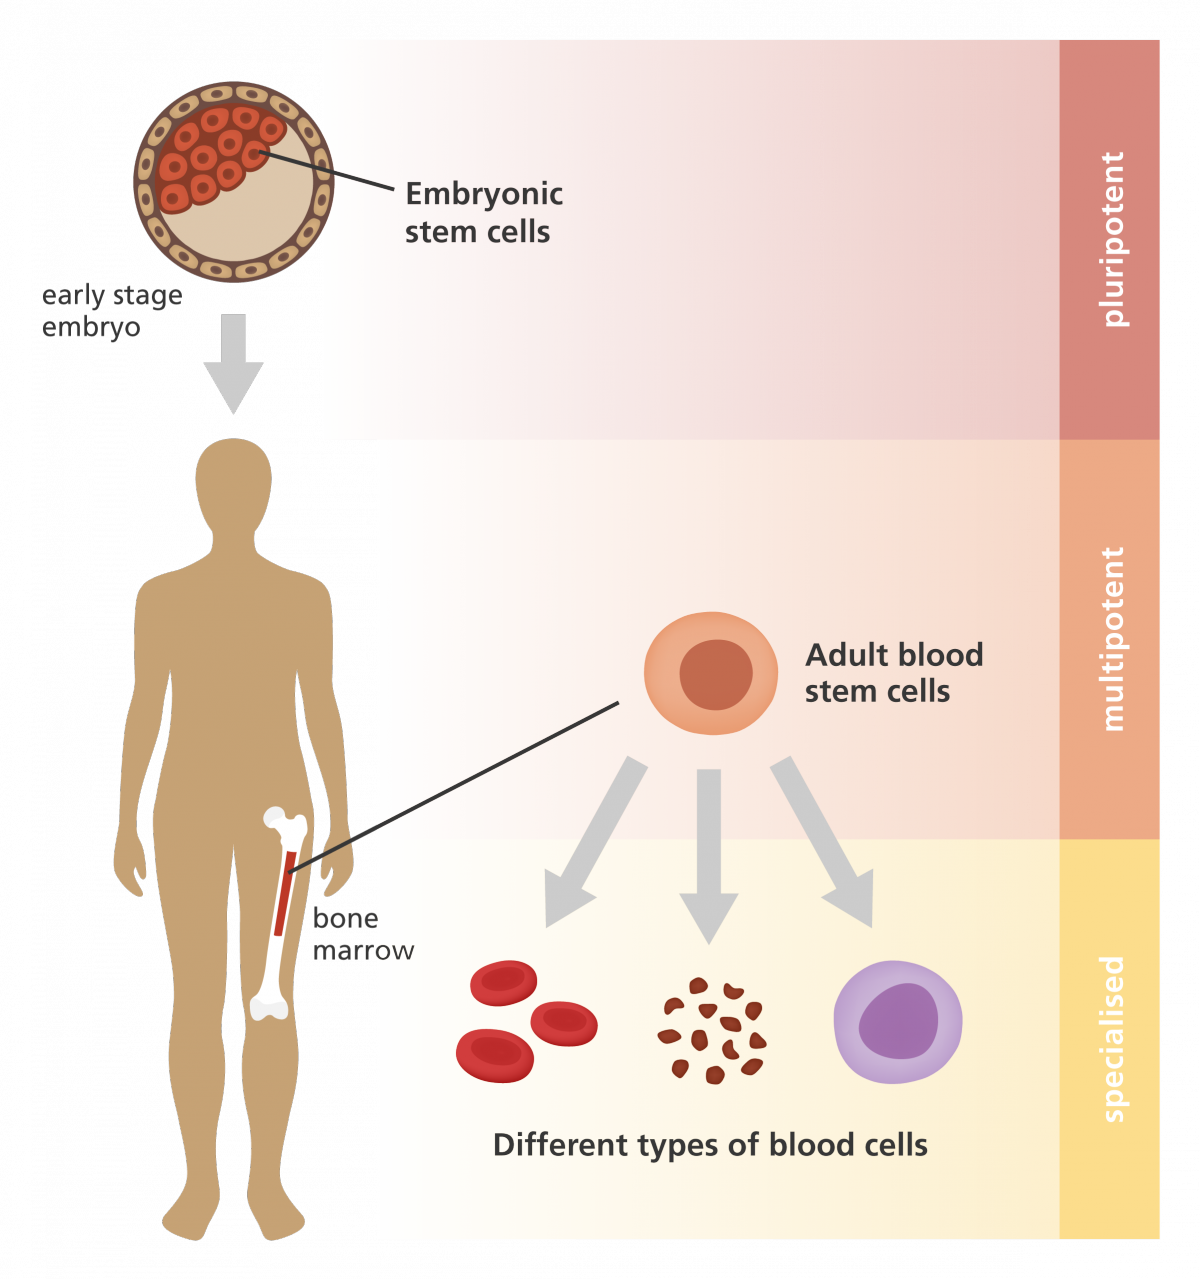
\includegraphics[width=0.6\textwidth]{../figures/stem cells.png}
    \caption{Stem Cells}
    \label{fig:stem-cells}
\end{figure}

\begin{note}{ }
    Embryonic stem cells are right after fertilization.
\end{note}

\subsection{Stem Cell Transplant}
\begin{definition}[Stem Cell Transplant]
    Stem Cell Transplant replaces stem cells from a donor and is performed when a patient's stem cells or bone marrow have been damaged by disease, Chemotherapy, or radiation therapy. 
\end{definition}

Stem cells can be collected from the: 
\begin{itemize}
    \item{Bone marrow}
    \item{Peripheral blood}
    \item{Umbilical cord}
\end{itemize}

\begin{figure}[!htb]
    \centering
    \subfloat[\centering Bone marrow biopsy]{{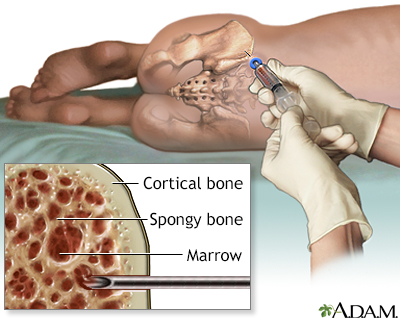
\includegraphics[width=0.45\textwidth]{../figures/bone marrow.jpg}}}  
    \qquad
    \subfloat[\centering Bone marrow stem cells]{{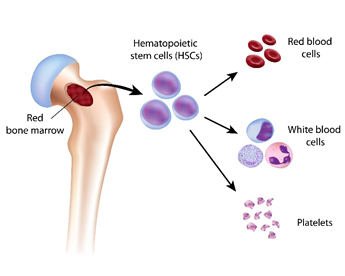
\includegraphics[width=0.45\textwidth]{../figures/bone marrow stem cells.jpg}}}
    \label{fig:example}
\end{figure}

\section{Hiearchy of an Organism}
\begin{definition}[Hiearchy of an Organism]
    The hiearchy is 
    \[
        \text{cell}\to \text{tissue}\to \text{organ}\to \text{system}\to \text{organism}
    \]
    See Figure \ref{fig:hierachy}.
\end{definition}

\begin{figure}[H]
\centering
    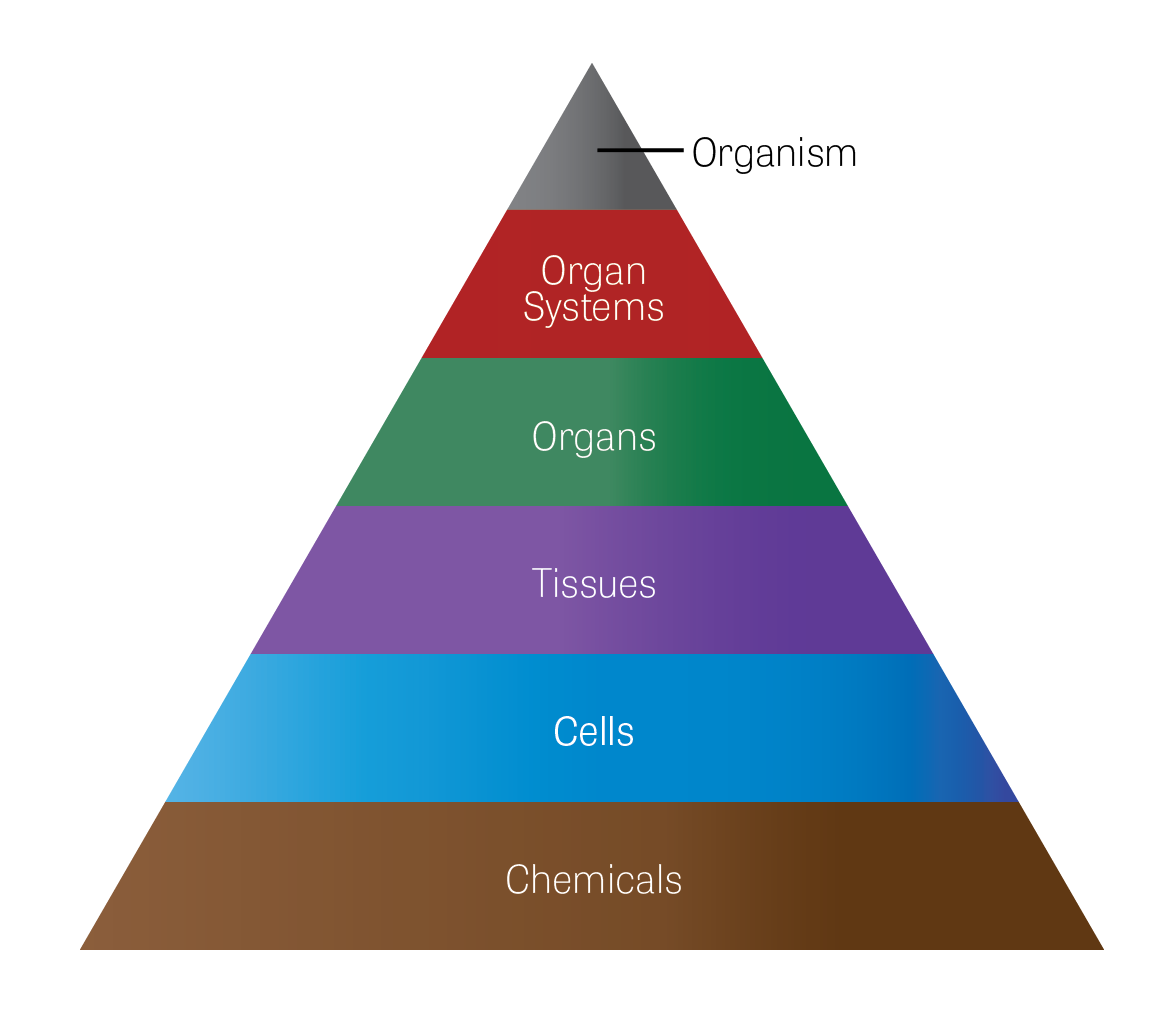
\includegraphics[width=0.5\textwidth]{../figures/hiearchy.png}
    \caption{Hiearchy of an Organism}
    \label{fig:hierachy}
\end{figure}

\begin{enumerate}
\setlength\itemsep{0.5em}
    \item{Cellular level heart muscle cell.}
    \item{Tissue level heart muscle tissue.}
    \item{Organ level heart.}
    \item{Organ system level circulatory system.}
    \item{Organism level deer.}
\end{enumerate}
\invis
\begin{itemize}
    \item{ \textbf{Cell}: the smallest function unit of an organism.}
    \item{ \textbf{Tissue}: a group of cells that perform a similar limited function.}
        \begin{itemize}
            \item{Four main types: epithelial, connective, muscle, and nerve tissue}
        \end{itemize}
    \item{ \textbf{Organ}: a structure composed of different tissues to perform a complex function.}
    \item{ \textbf{Organ system}: a system of one or more organs that work together to perform a vital body function.}
\end{itemize}

\section{Types of Tissues}
\subsection{Epithelial Tissue}
\begin{definition}[Epithelial Tissue]
    A thin sheet that covers body surfaces and lining the internal organs.
\end{definition}

\begin{itemize}
    \item{Skin and lining of the digestive system.}
    \item{Protection from hydration.}
    \item{Low friction surfaces.}
\end{itemize}

\subsection{Connective Tissue}
\begin{definition}[Connective Tissue]
    Connective tissue are various types of cells and fibres held together by a liquid, solid, or a gel, known as a matrix.
\end{definition}

\begin{itemize}
    \item{Bones, tendons, and blood.}
    \item{\textbf{Provides support and insulation.}}
\end{itemize}

\subsection{Muscle Tissue}
\begin{definition}[Muscle Tissue]
    Muslce tissue contains proteins like actin and myosin that can contract and move.
\end{definition}

\begin{itemize}
    \item{Muscles that make bones move.}
    \item{Muscles surrounding the digestive tract.}
    \item{Heart.}
        \divider
    \item{Bundles of long cells called muscle fibres that contain specialized proteins capable of shortening or contracting.}
        \divider
    \item{Movement.}
\end{itemize}

\subsection{Nerve Tissue}
\begin{definition}[Nerve Tissue]
    Nerve tissue conducts electrical signals from one part of the body to another.
\end{definition}

\begin{itemize}
    \item{Brain.}
    \item{Nerves in sensory organs.}
        \divider
    \item{Long, thin cells with fine branches at the ends capable of conducting elelectrical impulses.}
        \divider
    \item{Sensory.}
    \item{Communication within the body.}
    \item{Coordination of body functions.}
\end{itemize}

% YESTERYDAY
\section{Stem Cells Case Study Mini-Assignment}
\begin{enumerate}
\setlength\itemsep{0.5em}
    \item{What is the difference between embryonic stem cells adn adult stem cells?}
    \begin{solution}
        Embryonic stem cells:
        \begin{itemize}
            \item{Embryonic stem cells exist only right after the fertilization of an egg.}
            \item{Embryonic stem cells can specialize into any kind of body cell, be it epithelial cell, a red blood cell, nerve cell, bone cell, etc.}
            \item{Adults don't have embryonic stem cells.}
        \end{itemize}
        Adult stem cells:
        \begin{itemize}
            \item{Adult blood stem cells are located in the bone marrow AND in the peripheral blood.}
            \item{Adult blood stem cells can only differentiate into either red blood cells, white blood cells, or platelets.}
        \end{itemize}
    \end{solution}

    \item{Based on the article, how would you describe what cancer is?}
    \begin{solution}
            As a result of some kind of mutation in the cellular DNA, this causes healthy cell checkpoints to become dysfunctional and causes uncontrollable cell growth/division. This uncontrollable growth eventually materializes as a tumor in the healthy tissue
    \end{solution}

    \item{Conduct some research on the following cancer treatments: chemotherapy, radiation, therapy, and surgery. Do you think that differentiation therapy has any benefits over these known treatments? Explain your reasoning.}
        \begin{solution}
            \invis
            \begin{itemize}
                \item{Chemotherapy is targeted to kill cancer cells, but in the administration of chemotherapy, the drugs are targeting the healthy cells as well. Though chemotherapy may be effective in killing the cancer cells, it also damages healthy cells, which can lead to adverse effects such as nausea, hair loss, and cdecreasing in immune function.}
                \item{Radiation therapy, uinless specifically localized, can also have adverse effects on surrounding healthy tissue.}
                \item{Differentiation therapy is much more targeted towards turning cancer cells back into normal cells, so the use of toxic chemical is not necessary. This can decrease the number of adverse effects as well as results of this treatment.}
            \end{itemize}
            With this new kind of treatment, it could open many doors to groundbreaking cancer research and therapy; possible high mobilization of this particular kind of research (can lead to scientific discoveries).
        \end{solution}
\end{enumerate}

\section{Digestive System}
\begin{definition}[Digestive System]
    The digestives system is the organ system responsible for breaking up and digesting food, and secreting waste. The digestive tract is lined with epithelial tissue, goblet cells that release mucous, connective tissue, muscles, and nerves. See Figure \ref{fig:digestive-system}.
\end{definition}

\begin{figure}[H]
\centering
    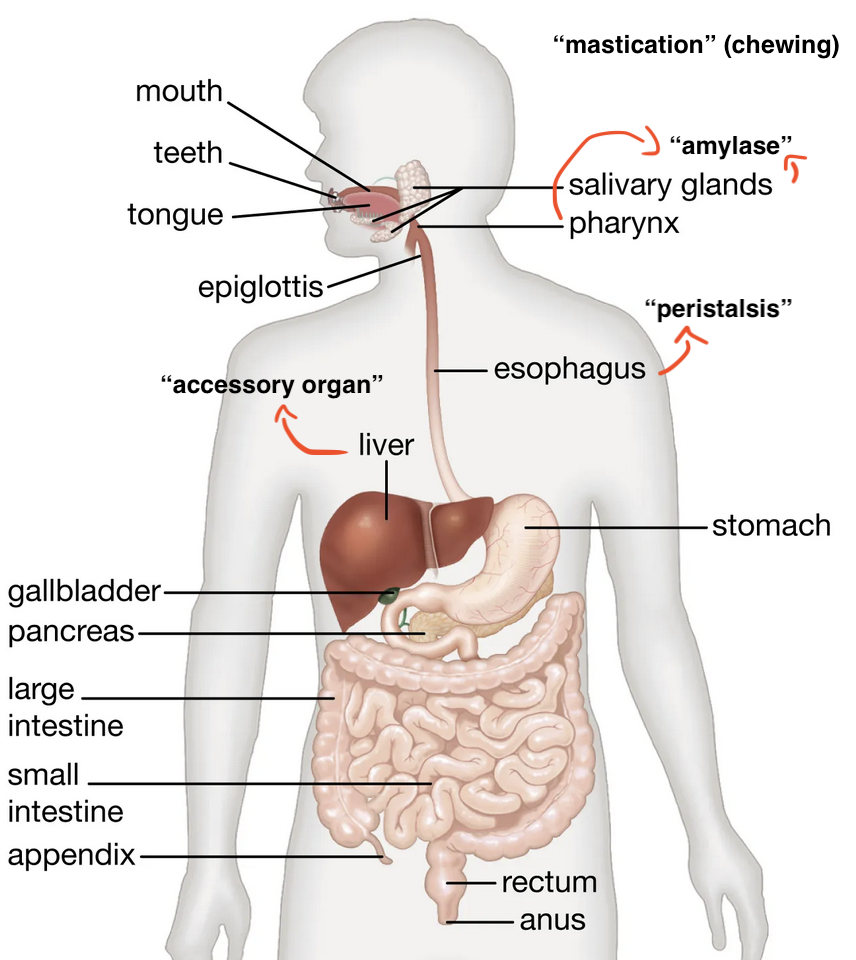
\includegraphics[width=\textwidth]{../figures/digestive system}
    \caption{The digestive system.}
    \label{fig:digestive-system}
\end{figure}

\subsection{Mouth}
\begin{definition}[Mouth]
    The mouth is where food enters and undergoes mechanical breakdown (mastication) and chemical breakdown through the saliva to form a bolus. The \textbf{bolus} is a ball-like mixture of food and saliva.
\end{definition}

\subsection{Esophagus}
\begin{definition}[Esophagus]
    A muscular tube that contracts through \textbf{peristalsis} to move the bolus to the stomach. See Figure \ref{esophagus-bolus}.
\end{definition}

\begin{figure}[H]
\centering
    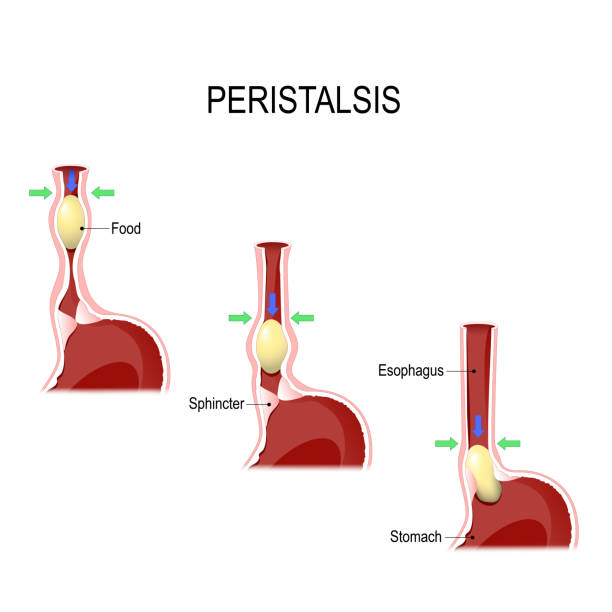
\includegraphics[width=\textwidth]{../figures/esophagus bolus.jpg}
    \caption{Peristalsis the \textbf{smooth muscles} create a pinch that pushes the bolus down into the stomach..}
    \label{esophagus-bolus}
\end{figure}

\subsection{Epiglottis}
\begin{definition}[Epiglottis]
    Is a flap that seals off the trachea during swalloing to direct the bolus to the esophagus.
\end{definition}

\subsection{Stomach}
\begin{definition}[Stomach]
    A J-shaped organ that holds, churns, and adds acids and enzymes to turn the bolus into \textbf{chyme}. Chyme is the partially digested food that contains acids and enzymes. See Figure \ref{fig:stomach}.
\end{definition}

\begin{figure}[H]
\centering
    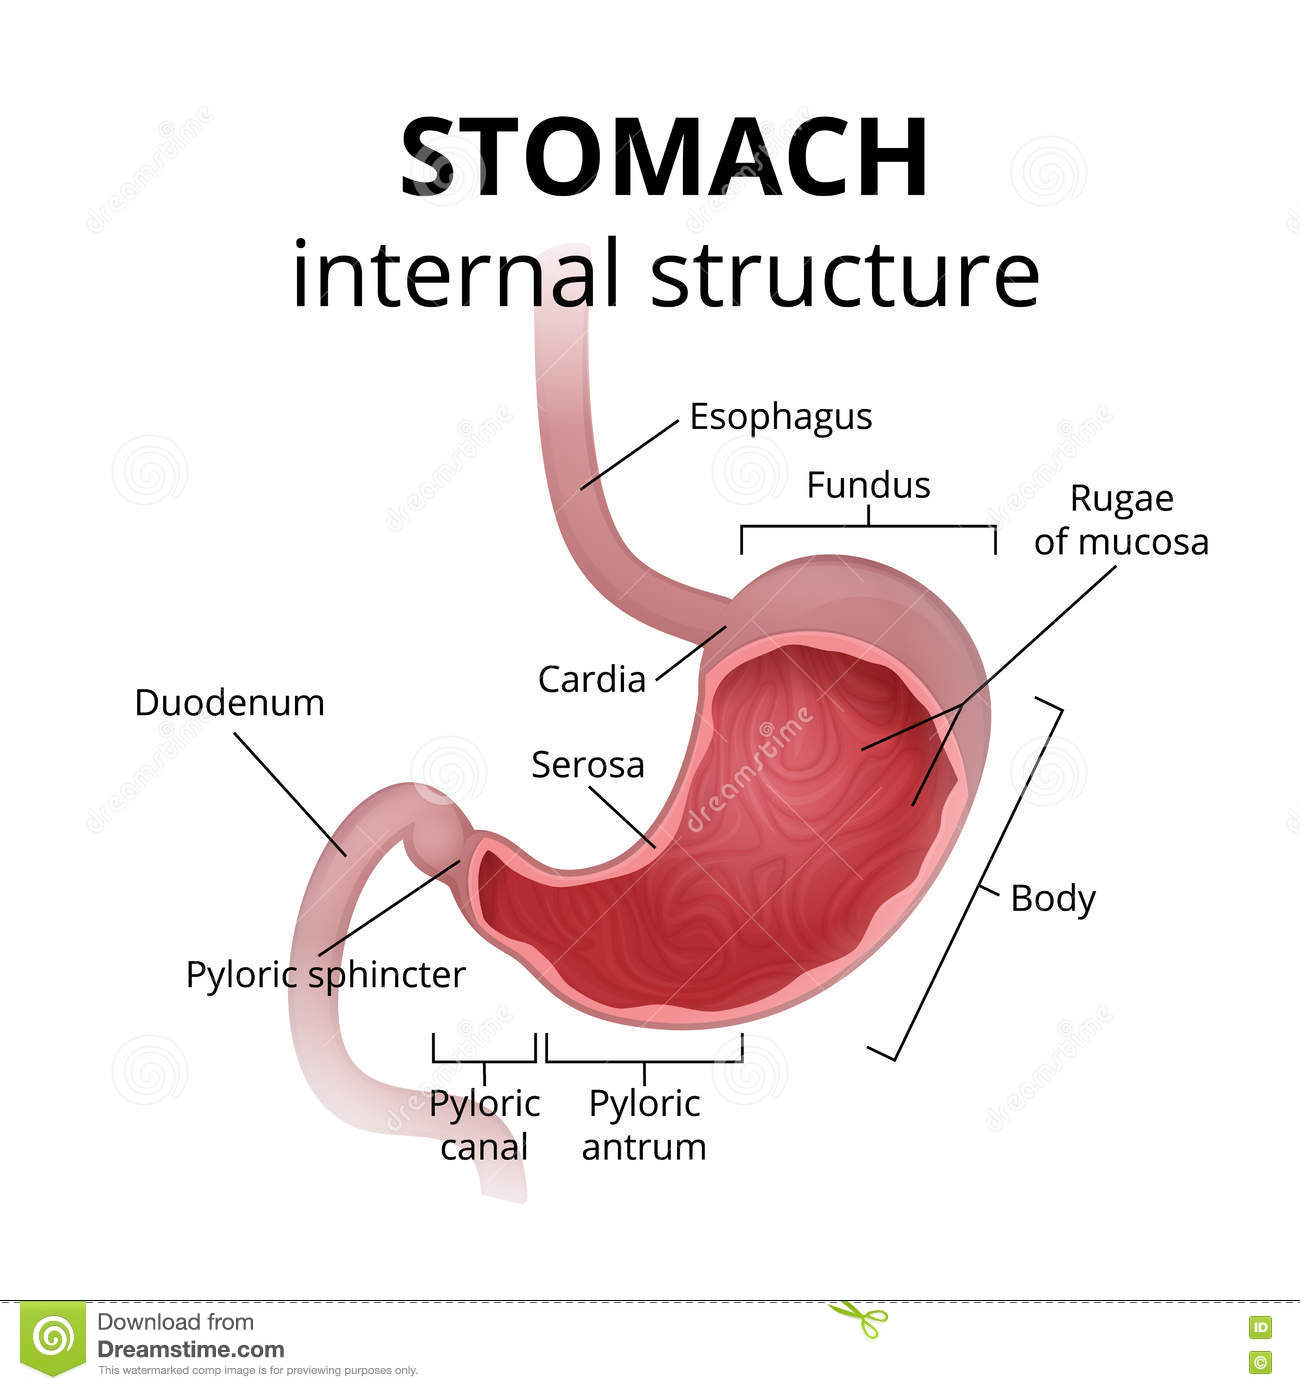
\includegraphics[width=0.6\textwidth]{../figures/stomach}
    \caption{The stomach.}
    \label{fig:stomach}
\end{figure}

\subsection{Small Intestine}
\begin{definition}[Small Intestine]
    The small intestine continues to digest and is the main site of absorption of nutrients. Consists of \textbf{villi} and \textbf{microvilli} to increase surface area for absorption. See Figure \ref{fig:small-intestine}.
\end{definition}

\begin{figure}[H]
\centering
    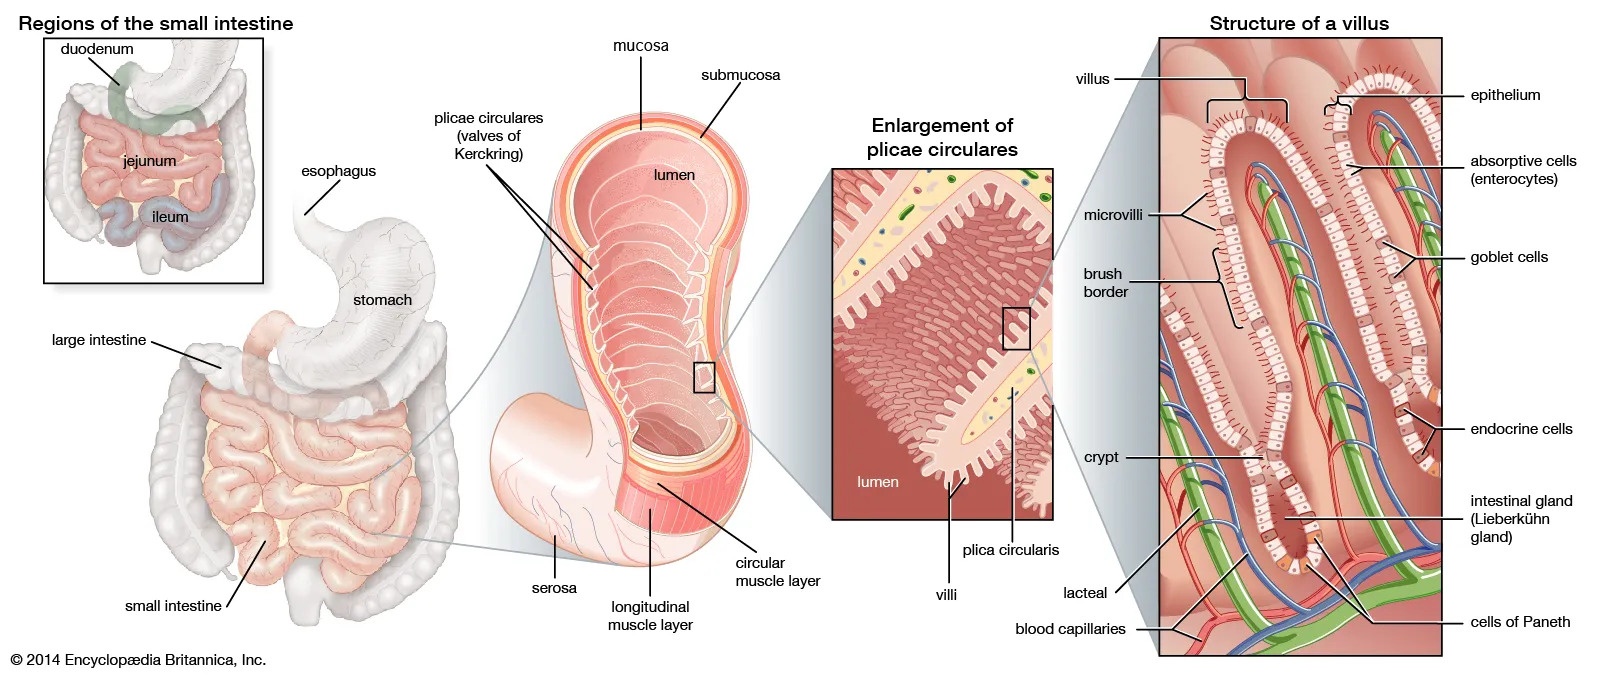
\includegraphics[width=\textwidth]{../figures/small intestine.jpg}
    \caption{The small intestine have small villi and further microvilli which ensures that you obtain all the nutrients from the food.}
    \label{fig:small-intestine}
\end{figure}

\subsection{Large Intestine}
\begin{definition}[Large Intestine]
    Aprobiotic environment that mainly absorbs water and minerals.
\end{definition}

\subsection{Appendix}
\begin{definition}[Appendix]
    May house beneficial gut bacteria.
\end{definition}

\subsection{Rectum}
\begin{definition}[Rectum]
    The end of the large intestine that temprarily stores feces.
\end{definition}

\subsection{Anus}
\begin{definition}[Anus]
    An opening where feces is excreted.
\end{definition}

\divider

\subsection{Accessory Organs: Liver}
\begin{definition}[Liver]
    Produces digestive enzymes and bile; also removes toxins from the blood. See Figure \ref{fig:accessory-organs}.

\end{definition}

\subsection{Gall Bladder}
\begin{definition}[Gall Bladder]
    Stores the bile, which is used to emsulify fats. See Figure \ref{fig:accessory-organs}.
\end{definition}

\subsection{Pancreas}
\begin{definition}[Pancreas]
    Produces insulin, which is a hormone that regulates blood glucose concentration after a meal. See Figure \ref{fig:accessory-organs}.
\end{definition}

\begin{figure}[H]
\centering
    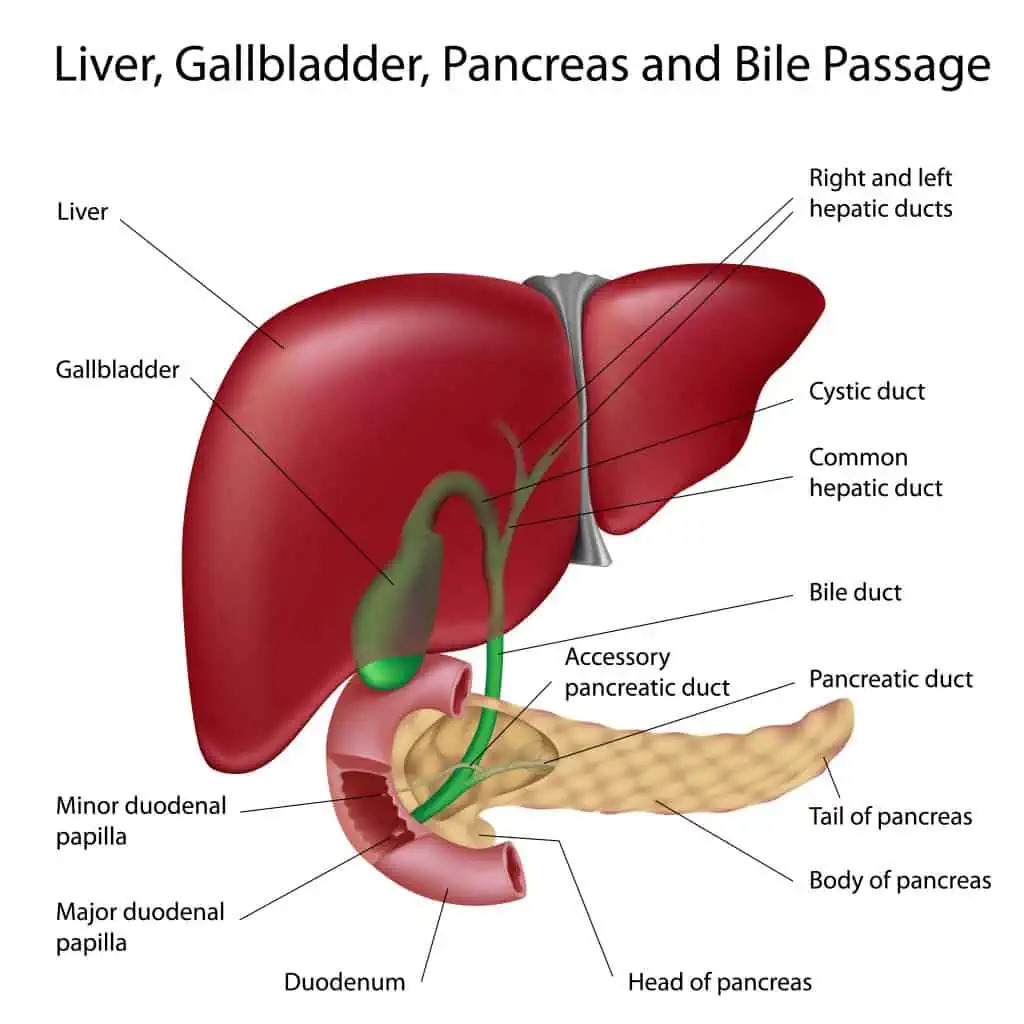
\includegraphics[width=0.6\textwidth]{../figures/accessory organs.jpg}
    \caption{The accessory organs: the liver, gall bladder, and pancreas.}
    \label{fig:accessory-organs}
\end{figure}

% TODAY 
\subsection{Diseases of the Digestive System}
\begin{table}[h!]
    \renewcommand{\arraystretch}{1.5}
    \setlength{\tabcolsep}{10pt}
    \setlength{\arrayrulewidth}{0.25mm}

    \begin{center}
        \vspace{0.5em}
        \begin{tabular}{|l|l|}
        \hline
         & Gastroesophageal Reflux Disease (GERD) \\ 
        \hline
        Description & Irration of the esopghageal lining due to acid from the stomach. \\
        \hline
        Symptoms & Heartburn, chest pain, bitter taste\\ 
        \hline 
        Causes & Weakening or abnormalities of the esopghageal sphincter\\ 
        \hline 
        Treatment & Antacids, drugs to reduce acid production, surgery\\
        \hline
        \end{tabular}
    \end{center}
\end{table}

\begin{table}[h!]
    \renewcommand{\arraystretch}{1.5}
    \setlength{\tabcolsep}{10pt}
    \setlength{\arrayrulewidth}{0.25mm}

    \begin{center}
        \vspace{0.5em}
    \begin{tabular}{|l|l|}
        \hline
         & Gastric Ulcer \\ 
        \hline
        Description & Open sores that develop in the stomach lining \\
        \hline
        Symptoms & Stomach pain, vomiing blood, dark blood in stool\\ 
        \hline 
        Causes & Helicobacter pylori infection NSAIDS (i.e. ibuprofen)\\ 
        \hline
        Treatment & Antibiotics if H. pyroli infection, alternative medication\\ 
        \hline
        \end{tabular}
    \end{center}
\end{table}

\section{Circulatory System}
\begin{definition}[Circulatory System]
    The organ system responsible for the 
    \begin{itemize}
        \item{Delivery of nutrients and gases.}
        \item{Regulation of body temperature.}
        \item{Defense against invading organisms.}
    \end{itemize}
    \textbf{Components:}
    \begin{itemize}
        \item{Heart.}
        \item{Blood vessels.}
        \item{Blood.}
    \end{itemize}
\end{definition}

\subsection{Heart}
\begin{definition}[Heart]
    A pump that distributes nutrients and gases to every cell in the body. The heart is composed of three kinds of tissues: 
    \begin{itemize}
        \item{ \textbf{Cardiac muscle tissue} contracts synergistically (at the same time) to pump blood throughout the body.}
        \item{ \textbf{Nerve tissue} is responsible for the heart rate and can respond to stress, temperature, and physical activity.}
        \item{ \textbf{Epithelial tissue} lines the inner surface of the heart to allow blood to flow freely; smooth layer of epithelial tissue on the outside reduces friction and protects the heart from damage.}
    \end{itemize}
\end{definition}

\subsection{Blood vessels}
\begin{definition}[Blood vessels]
    There are three kinds of blood vessels: 
    \begin{itemize}
        \item{ \textbf{Artery} carries blood away from the heart; have thick, muscular walls to withstand high blood pressure. See Figure \ref{fig:artery}.}
        \item{ \textbf{Vein} carries blood through the heart; have thinner walls with valves to pump blood back to the heart. See Figure \ref{fig:artery}.}
        \item{ \textbf{Capillary} connects arteries to veins; have one-cell thick walls to maximize diffusion of susbstance between blood and tissues. See Figure \ref{fig:capillary}.}
    \end{itemize}
\end{definition}

\begin{figure}[H]
\centering
    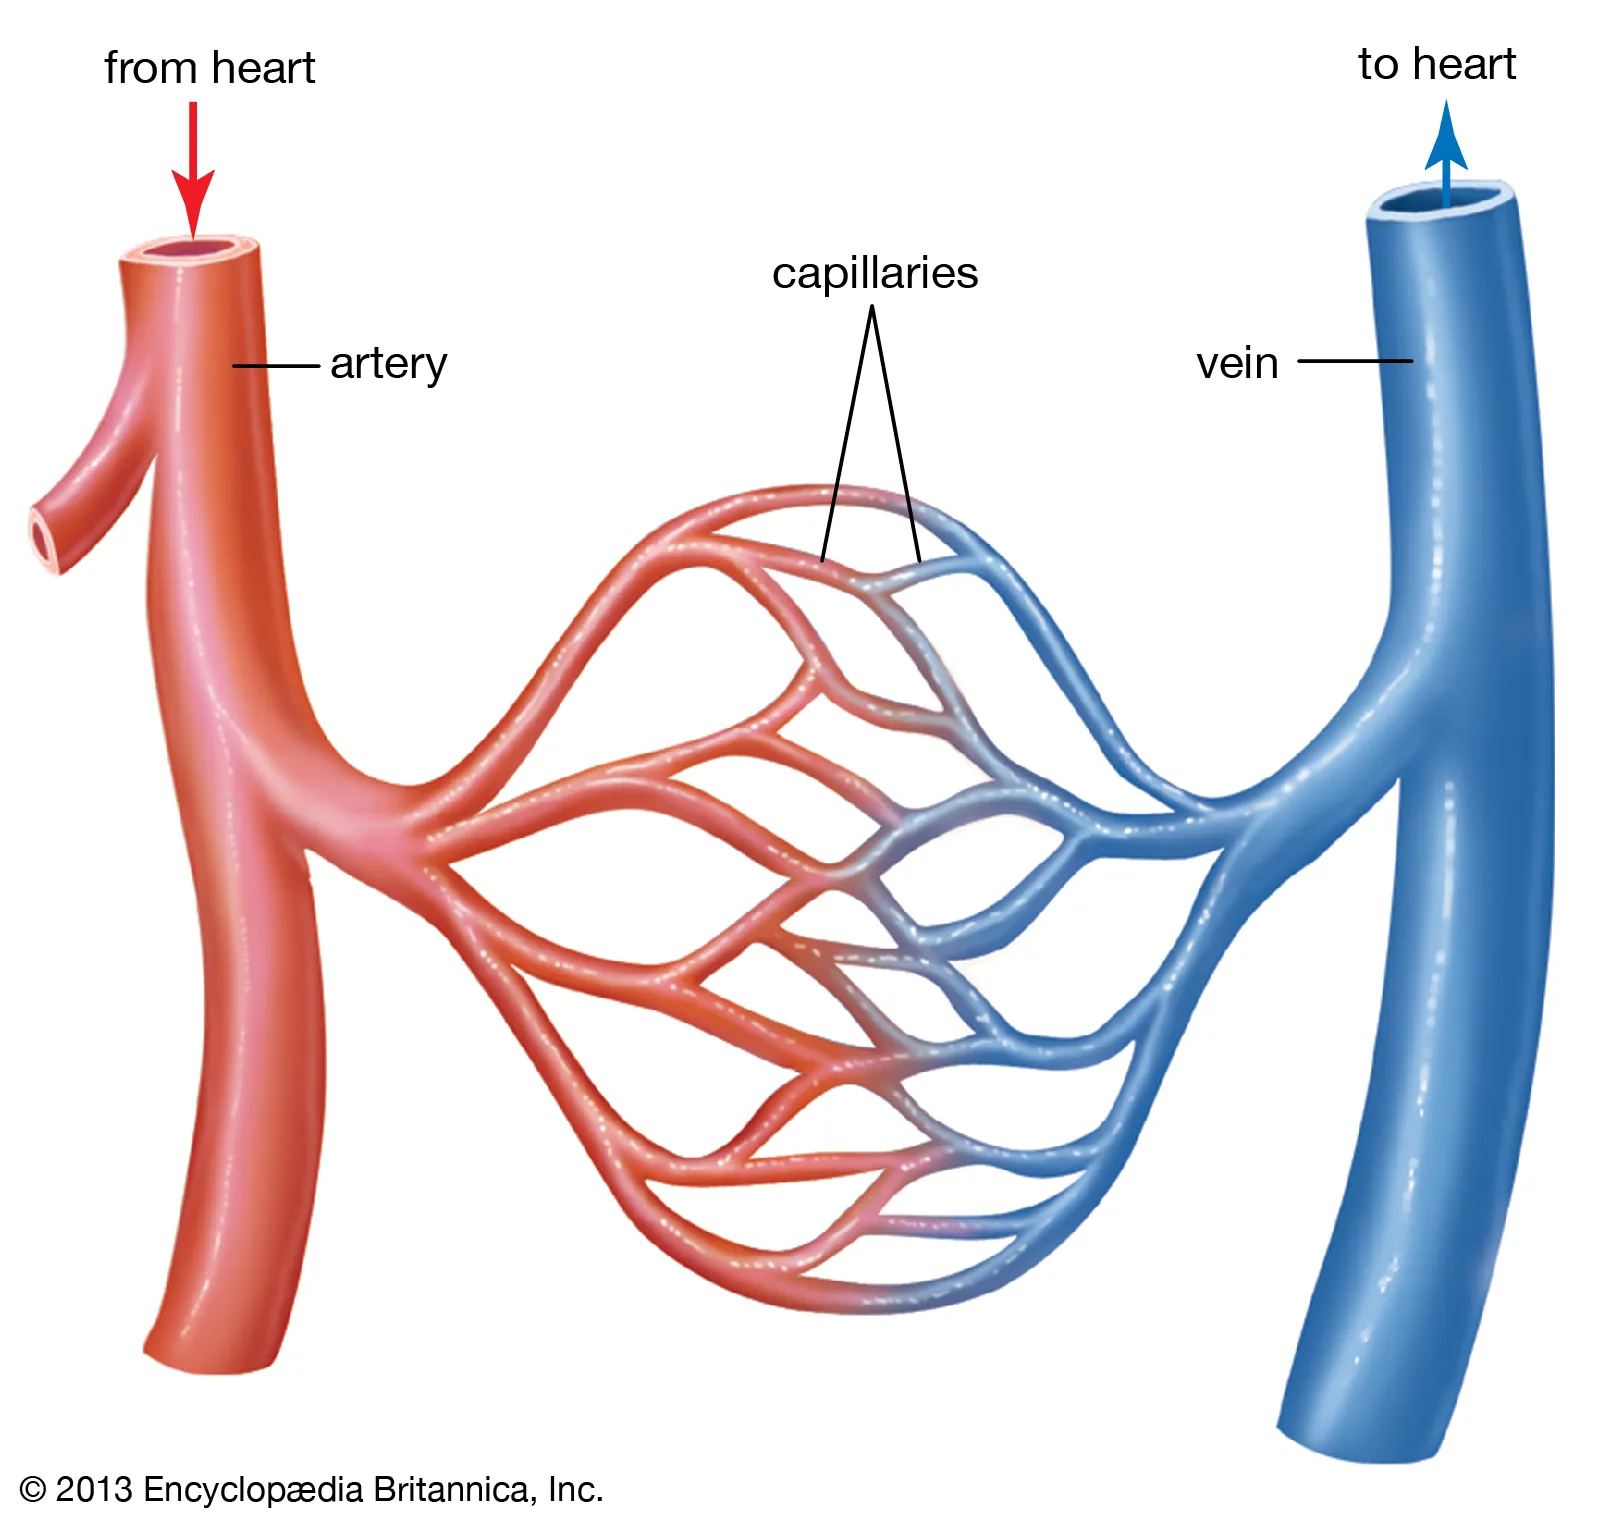
\includegraphics[width=0.5\textwidth]{../figures/artery.png}
    \caption{The artery (red) and the vein (blue). The connect part are referred as the capillaries.}
    \label{fig:artery}
\end{figure}

\begin{figure}[H]
\centering
    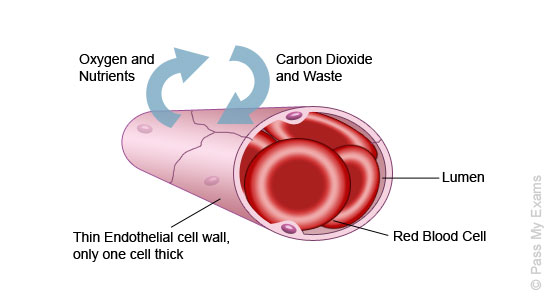
\includegraphics[width=0.7\textwidth]{../figures/capillary.jpg}
    \caption{The cappilary.}
    \label{fig:capillary}
\end{figure}

\subsection{Blood}
\begin{definition}[Blood]
    A connective tissue that consists of the following main cells: 
    \begin{itemize}
        \item{ \textbf{Erythrocytes} are red blood cells that are biconcave in shape and contain hemoglobin that attaches to oxyge and carbon dioxide.}
        \item{ \textbf{Leukocytes} are white blood cells that are defending the body against pahtogens.}
        \item{ \textbf{Platelets } help ion blood clotting.}
        \item{ \textbf{Plasma} is protein rich liquid that suspends the cells.}
    \end{itemize}
    See Figure \ref{fig:hemoglobin} and Figure \ref{fig:hematocrit}.
\end{definition}

% TODO 
% Side by side figures
\begin{figure}[H]
\centering
    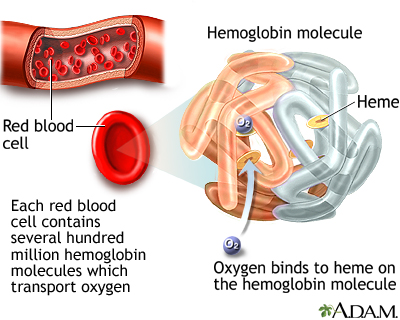
\includegraphics[width=0.5\textwidth]{../figures/hemloblogin.jpg}
    \caption{Hemoglobin.}
    \label{fig:hemoglobin}
\end{figure}

\begin{figure}[H]
\centering
    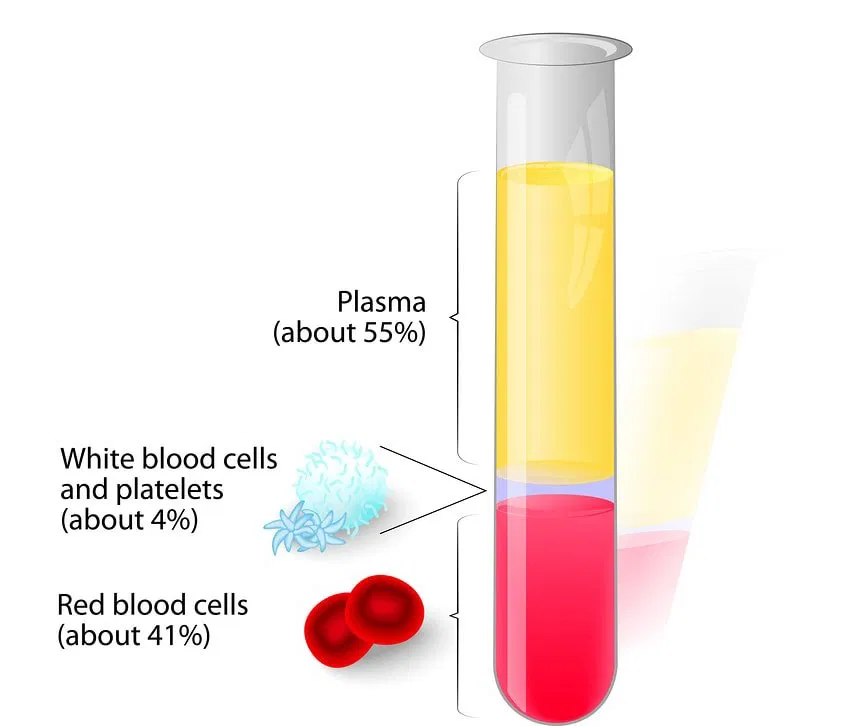
\includegraphics[width=0.5 \textwidth ]{../figures/hematocrit.png}
    \caption{A centrifuge for separating blood plasma. This is known as \textbf{hematocrit}.}
    \label{fig:hematocrit}
\end{figure}

\end{document}
